% v4 figures, generated by make_v4_figs.py from committed files
% (posthoc-mm-signal 8cb29f7: n_detail_games.csv, n_detail_spread.csv; N_CHECK.md / n_check.json 863eb69;
\begin{figure}[t]\centering
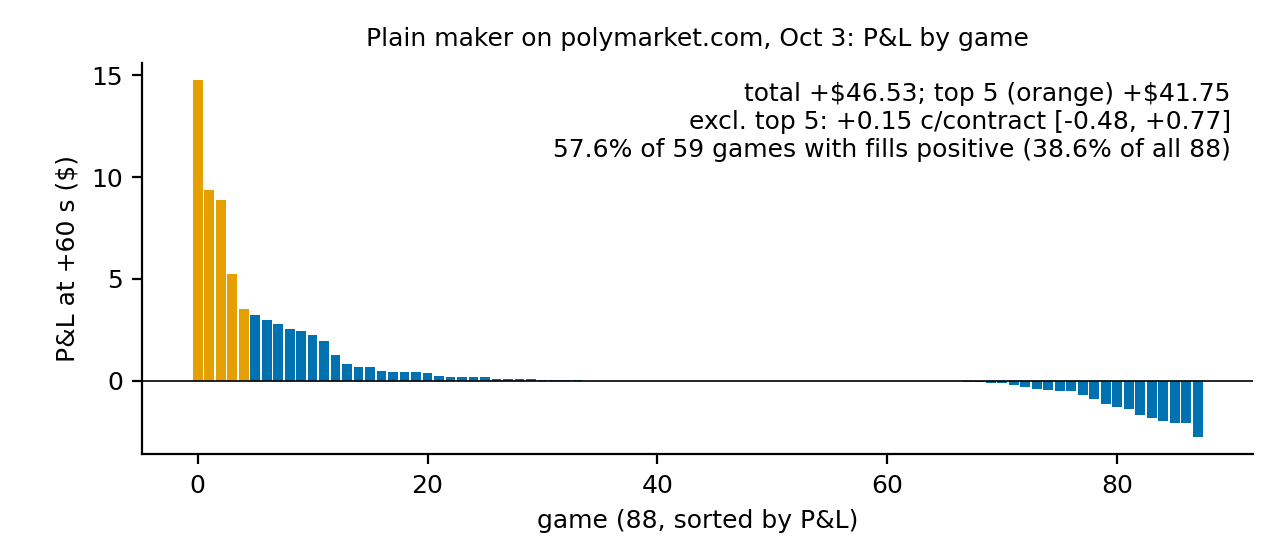
\includegraphics[width=\linewidth]{figs/v4_per_game.png}
\caption{Descriptive, one day (Oct 3, 88 games), simulated on recorded top of book, maker fee 0, not pre-registered.
Plain maker on polymarket.com (join best bid and ask, 10 contracts, inventory cap $\pm 50$, strict trade-through
fills): P\&L at +60 s per game, sorted; total +\$46.53, the five largest games in orange. Excluding the five largest
games: +0.15 c per contract [-0.48, +0.77] (N\_CHECK.md, 863eb69). Source: n\_detail\_games.csv, posthoc-mm-signal
(8cb29f7).}
\label{fig:v4pergame}
\end{figure}

\begin{figure}[t]\centering
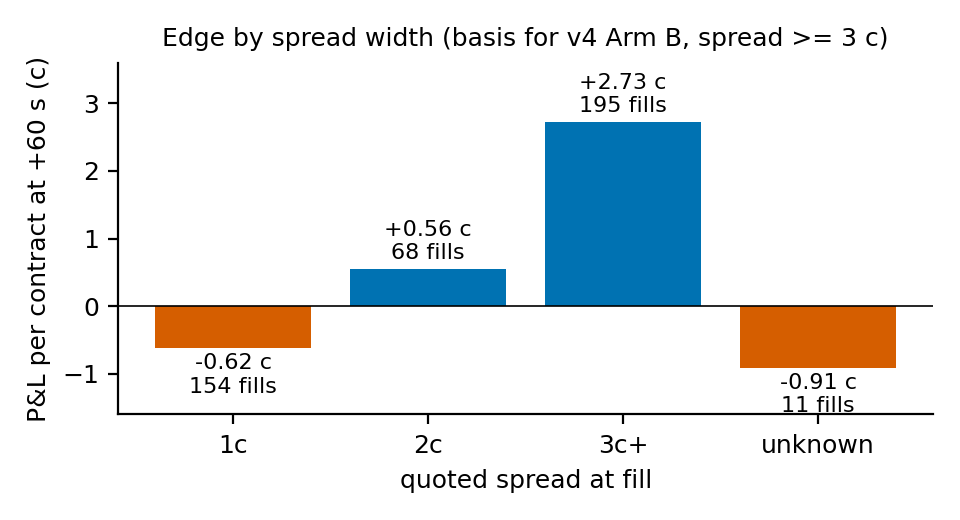
\includegraphics[width=0.9\linewidth]{figs/v4_spread.png}
\caption{Descriptive, one day (Oct 3, 88 games), simulated on recorded top of book, maker fee 0, not pre-registered.
P\&L per contract at +60 s by quoted spread at the fill: 1 c spreads lose (-0.62 c, 154 fills), 3 c and wider win
(+2.73 c, 195 fills). This motivates HYPOTHESIS\_v4 Arm B (quote only while the spread is at least 3 c). Source:
n\_detail\_spread.csv, posthoc-mm-signal (8cb29f7).}
\label{fig:v4spread}
\end{figure}

\begin{figure}[t]\centering
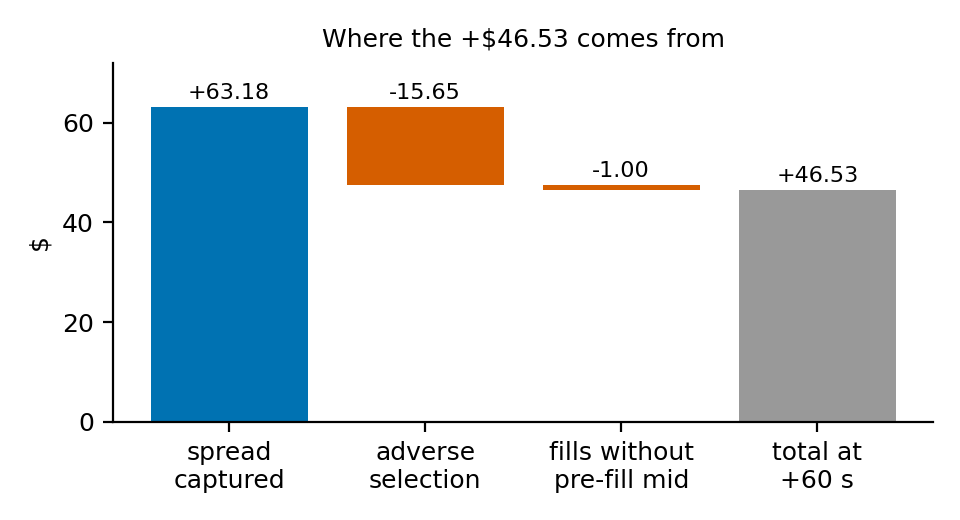
\includegraphics[width=0.9\linewidth]{figs/v4_decomp.png}
\caption{Descriptive, one day (Oct 3, 88 games), simulated on recorded top of book, maker fee 0, not pre-registered.
Split of the +60 s P\&L: spread captured +\$63.18 (388 fills with a mid just before the fill and at +60 s), adverse
selection (mid move from fill to +60 s) -\$15.65, and 2 fills without a pre-fill mid -\$1.00; total +\$46.53.
Source: N\_CHECK.md and n\_check.json (863eb69).}
\label{fig:v4decomp}
\end{figure}

